
\chapter{Pengenalan Enterprise Architecture}

\section{Definisi 'Enterprise'}

\subsection{Oxford English Dictionary}
Menurut Oxford English Dictionary, 'Enterprise' didefinisikan sebagai sebuah proyek atau usaha yang biasanya membutuhkan upaya dan keberanian. Selain itu, juga merujuk pada inisiatif, yaitu keberanian untuk mengambil risiko demi mendapatkan keuntungan, serta dapat diartikan sebagai organisasi atau perusahaan bisnis.

\subsection{Cambridge English Dictionary}
Menurut Cambridge English Dictionary, 'Enterprise' merujuk pada kemampuan untuk memikirkan rencana baru dan membuatnya berhasil. Selain itu, istilah ini juga digunakan untuk menggambarkan sebuah perusahaan.

\subsection{Merriam-Webster Dictionary}
Menurut Merriam-Webster Dictionary, 'Enterprise' adalah proyek atau usaha yang sering kali memerlukan keberanian. Definisi ini juga mencakup kesiapan untuk terlibat dalam usaha yang berani dan penuh risiko, serta menggambarkan suatu unit ekonomi yang terorganisir.

\subsection{Kesimpulan Definisi 'Enterprise'}
Secara umum, 'Enterprise' mengacu pada proyek atau usaha yang berani dan penuh risiko. Selain itu, istilah ini juga dapat merujuk pada organisasi atau perusahaan bisnis. Definisi ini secara umum konsisten di antara kamus bahasa Inggris terkemuka.

\section{Definisi 'Arsitektur'}

\subsection{Oxford English Dictionary}
Menurut Oxford English Dictionary, 'Arsitektur' didefinisikan sebagai seni atau praktik merancang dan membangun bangunan. Istilah ini juga dapat merujuk pada gaya atau metode konstruksi serta tata letak atau struktur dari suatu benda.

\subsection{Cambridge English Dictionary}
Menurut Cambridge English Dictionary, 'Arsitektur' adalah seni dan praktik merancang bangunan. Selain itu, istilah ini juga digunakan untuk menggambarkan gaya atau desain dari bangunan tertentu atau sekelompok bangunan, serta cara sesuatu diatur atau disusun.

\subsection{Merriam-Webster Dictionary}
Menurut Merriam-Webster Dictionary, 'Arsitektur' adalah seni atau ilmu dalam merancang dan membangun bangunan. Definisi ini juga mencakup metode atau gaya konstruksi, serta bagaimana bagian-bagian dari suatu objek diatur atau disistematisasi.

\subsection{Ringkasan Definisi 'Arsitektur'}
Secara umum, 'Arsitektur' merujuk pada seni atau praktik merancang dan membangun bangunan. Selain itu, istilah ini juga dapat merujuk pada gaya atau metode konstruksi, serta cara bagian-bagian dari sesuatu diatur atau disistematisasi.

\section{Definisi 'Arsitektur' Menurut IEEE}
Menurut IEEE, 'Arsitektur' adalah organisasi mendasar dari suatu sistem, yang melibatkan komponen sistem dan hubungan antar komponen. Arsitektur juga mencakup manajemen desain dan evolusi sistem, di mana komponen sistem dapat berupa perangkat keras, perangkat lunak, data, orang, dan proses.

\section{Definisi 'Enterprise Architecture'}

\subsection{Menurut Gartner}
Menurut Gartner, 'Enterprise Architecture' adalah disiplin untuk perancangan, perencanaan, pelaksanaan, dan pengendalian proyek. Disiplin ini membantu organisasi mencapai konsistensi antara bisnis dan IT serta melibatkan kolaborasi antara berbagai pemangku kepentingan. 'Enterprise Architecture' juga dapat digunakan untuk membantu dalam pengambilan keputusan strategis.

\subsection{Menurut TOGAF}
Menurut TOGAF, 'Enterprise Architecture' adalah kerangka arsitektur yang memberikan definisi dan desain dasar untuk arsitektur perusahaan. Tujuan dari arsitektur ini adalah untuk memastikan agar operasi perusahaan berjalan secara konsisten dan efisien dengan fokus pada standar dan prosedur yang digunakan di dalam perusahaan.

\subsection{Menurut ISO/IEC/IEEE 42010}
Menurut ISO/IEC/IEEE 42010, 'Enterprise Architecture' adalah pendekatan mendasar terhadap organisasi suatu sistem. Pendekatan ini melibatkan pemahaman semua komponen, hubungan antara komponen, serta lingkungan tempat komponen tersebut beroperasi. Pendekatan ini menekankan pentingnya struktur dan interaksi dalam suatu sistem, serta menyediakan kerangka kerja untuk pemahaman dan desain sistem.

\section{Berbagai Kerangka Arsitektur Enterprise}
Berbagai kerangka arsitektur enterprise telah muncul seiring waktu untuk memandu organisasi dalam menyusun sistem TI dan bisnis mereka. Beberapa kerangka yang terkenal termasuk Business System Planning (BSP), PRISM Architecture Framework, NIST Enterprise Architecture Model, Zachman Framework, Enterprise Architecture Planning (EAP), Sherwood Applied Business Security Architecture (SABSA), dan Federal Enterprise Architecture Framework (FEAF). Kerangka-kerangka ini bertujuan untuk membantu organisasi dalam mengelola kompleksitas sistem mereka, memastikan keselarasan antara tujuan bisnis dan TI.

Kerangka arsitektur enterprise lainnya termasuk Gartner's Enterprise Architecture Method, Department of Defense Architecture Framework (DoDAF), Australian Government AGA, Business Architecture Body of Knowledge (BizBoK), dan ISO Standard for Enterprise Modeling (ISO19439).

\section{Business System Planning (BSP)}
Business System Planning (BSP) melibatkan pemahaman tujuan bisnis, menganalisis proses bisnis, dan merancang arsitektur sistem informasi yang mendukung proses tersebut. BSP membantu organisasi untuk meningkatkan efisiensi, menyederhanakan operasi, dan mengoptimalkan alokasi sumber daya.

\begin{center}
	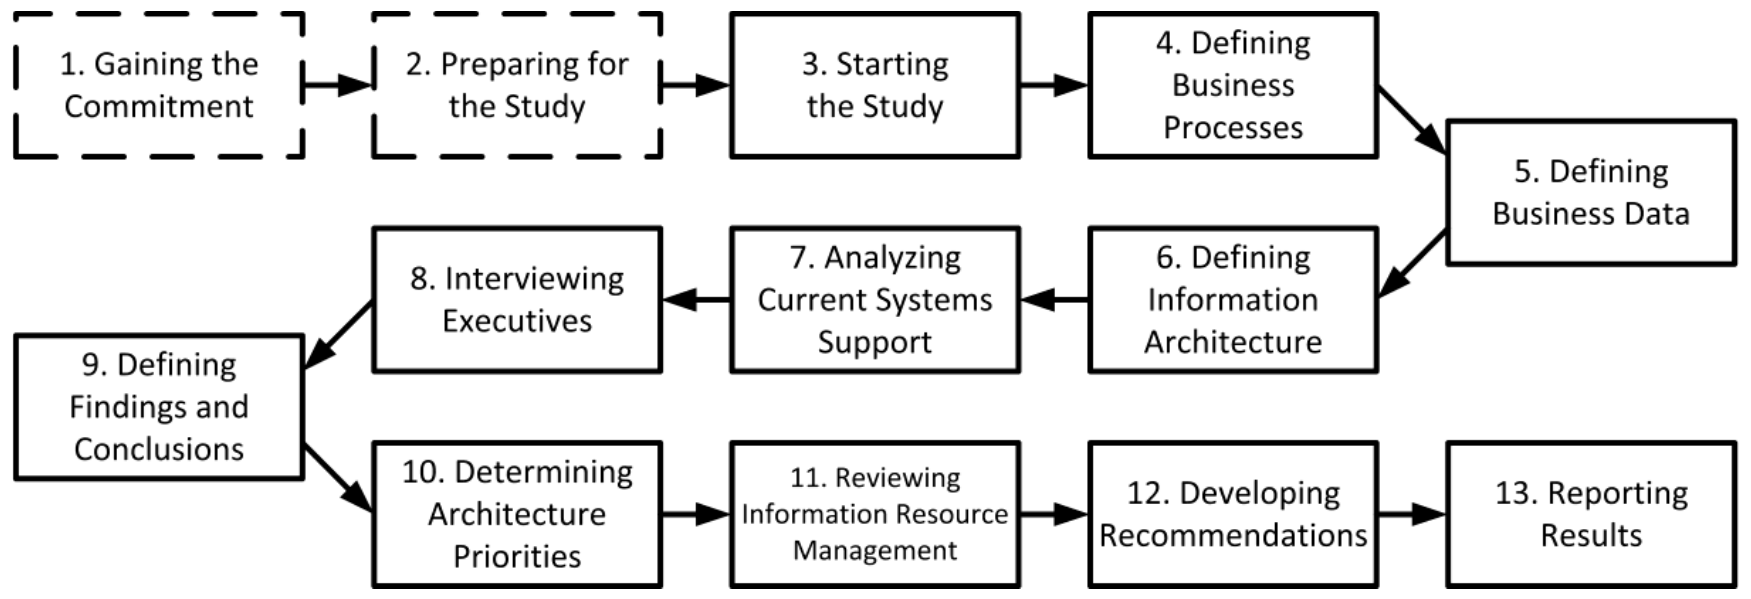
\includegraphics[width=\textwidth]{../figures/bsp}
\end{center}

\section{PRISM Architecture Framework}
PRISM Architecture Framework, atau Partnership for Research in Information Systems Management, merupakan salah satu kerangka arsitektur enterprise yang pertama kali dikembangkan oleh konsorsium vendor TI. Kerangka ini berfokus pada integrasi sistem dan teknologi informasi, membantu organisasi untuk memahami dan mengelola kompleksitas TI.

\begin{center}
	\begin{figure}[ht]
		\begin{minipage}[b]{0.49\linewidth}
			\centering
			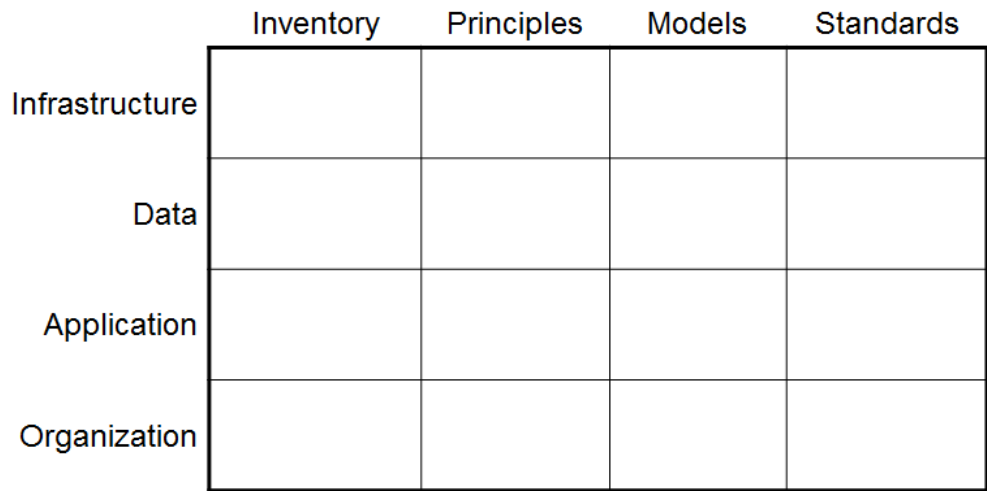
\includegraphics[width=\textwidth]{../figures/prism_matrix}
			\caption{matriks}
		\end{minipage}
		\hfill
		\begin{minipage}[b]{0.49\linewidth}
			\centering
			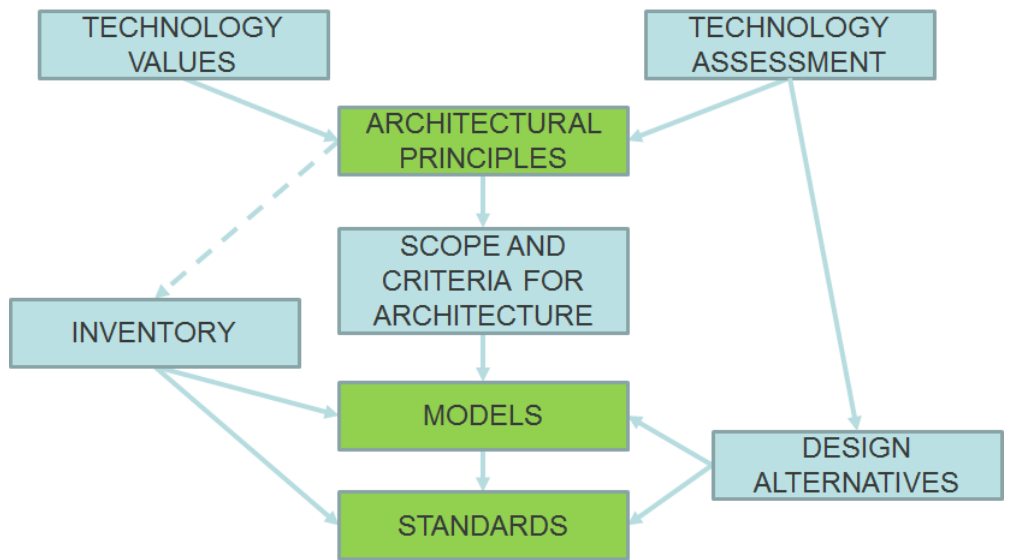
\includegraphics[width=\textwidth]{../figures/prism_relationships}
			\caption{hubungan}
		\end{minipage}
	\end{figure}
\end{center}

\section{NIST Enterprise Architecture Model}
Model Arsitektur Enterprise NIST, yang dikembangkan oleh National Institute of Standards and Technology, menekankan pada pengaturan dan organisasi operasi TI. Model ini membagi arsitektur TI menjadi lima tingkat yang meliputi bisnis, data, aplikasi, teknologi, dan hasil. Ini memungkinkan perencanaan strategis dan pengambilan keputusan berbasis data.

\begin{center}
	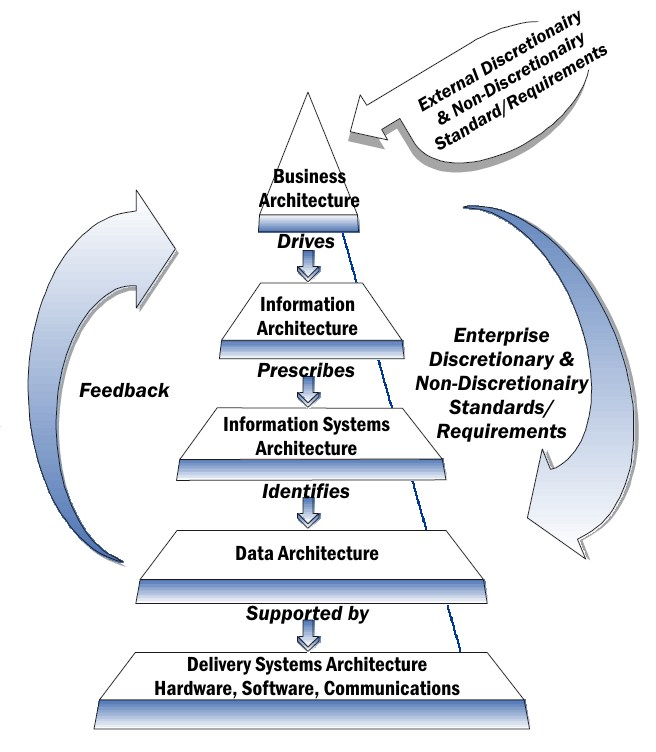
\includegraphics[width=.40\textwidth]{../figures/nist}
\end{center}

\section{Zachman Framework}
Zachman Framework adalah skema untuk memahami dan mengelola kompleksitas arsitektur enterprise, dibagi menjadi enam tingkat berbeda. Framework ini merangkum dari tingkat yang paling abstrak hingga yang paling konkret, cocok untuk berbagai jenis organisasi, dari bisnis hingga pemerintah.

\begin{center}
	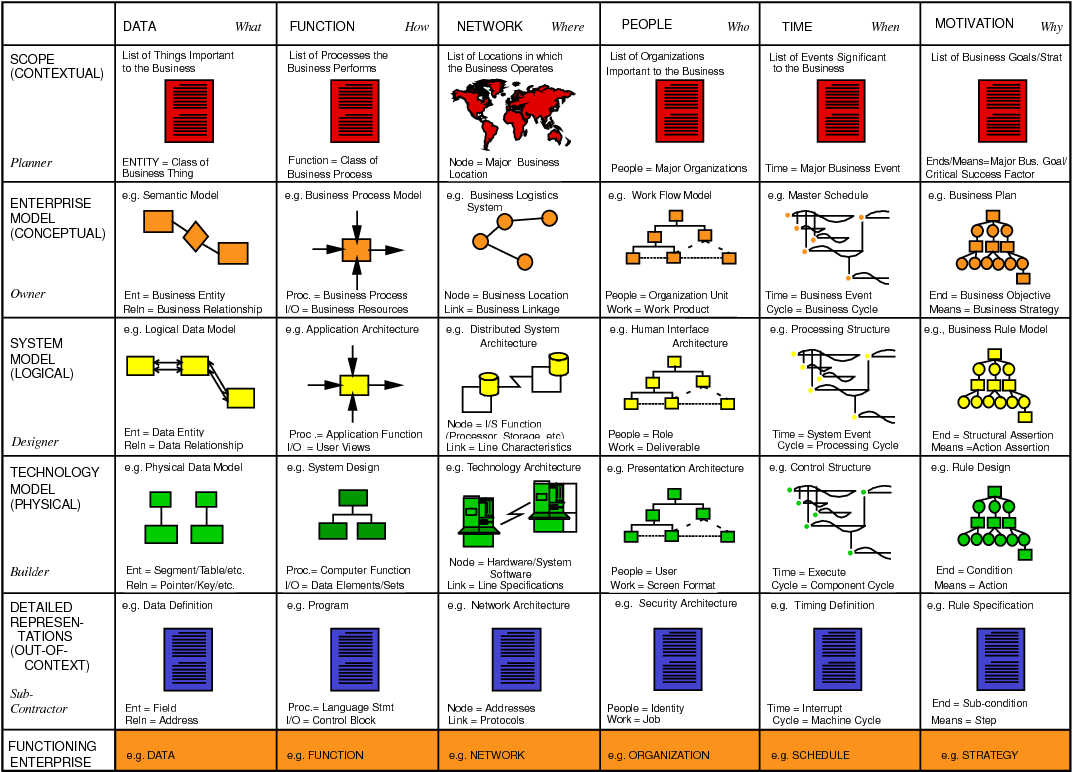
\includegraphics[width=0.76\textwidth]{../figures/zachman}
\end{center}

\section{Enterprise Architecture Planning (EAP)}
Enterprise Architecture Planning (EAP) mencakup metode perencanaan arsitektur sistem informasi. EAP bertujuan untuk mengidentifikasi kebutuhan bisnis dari teknologi informasi dan mengembangkan rencana untuk implementasi teknologi baru berdasarkan kebutuhan tersebut. Ini dapat membantu dalam transformasi digital dan perubahan organisasi.

\begin{center}
	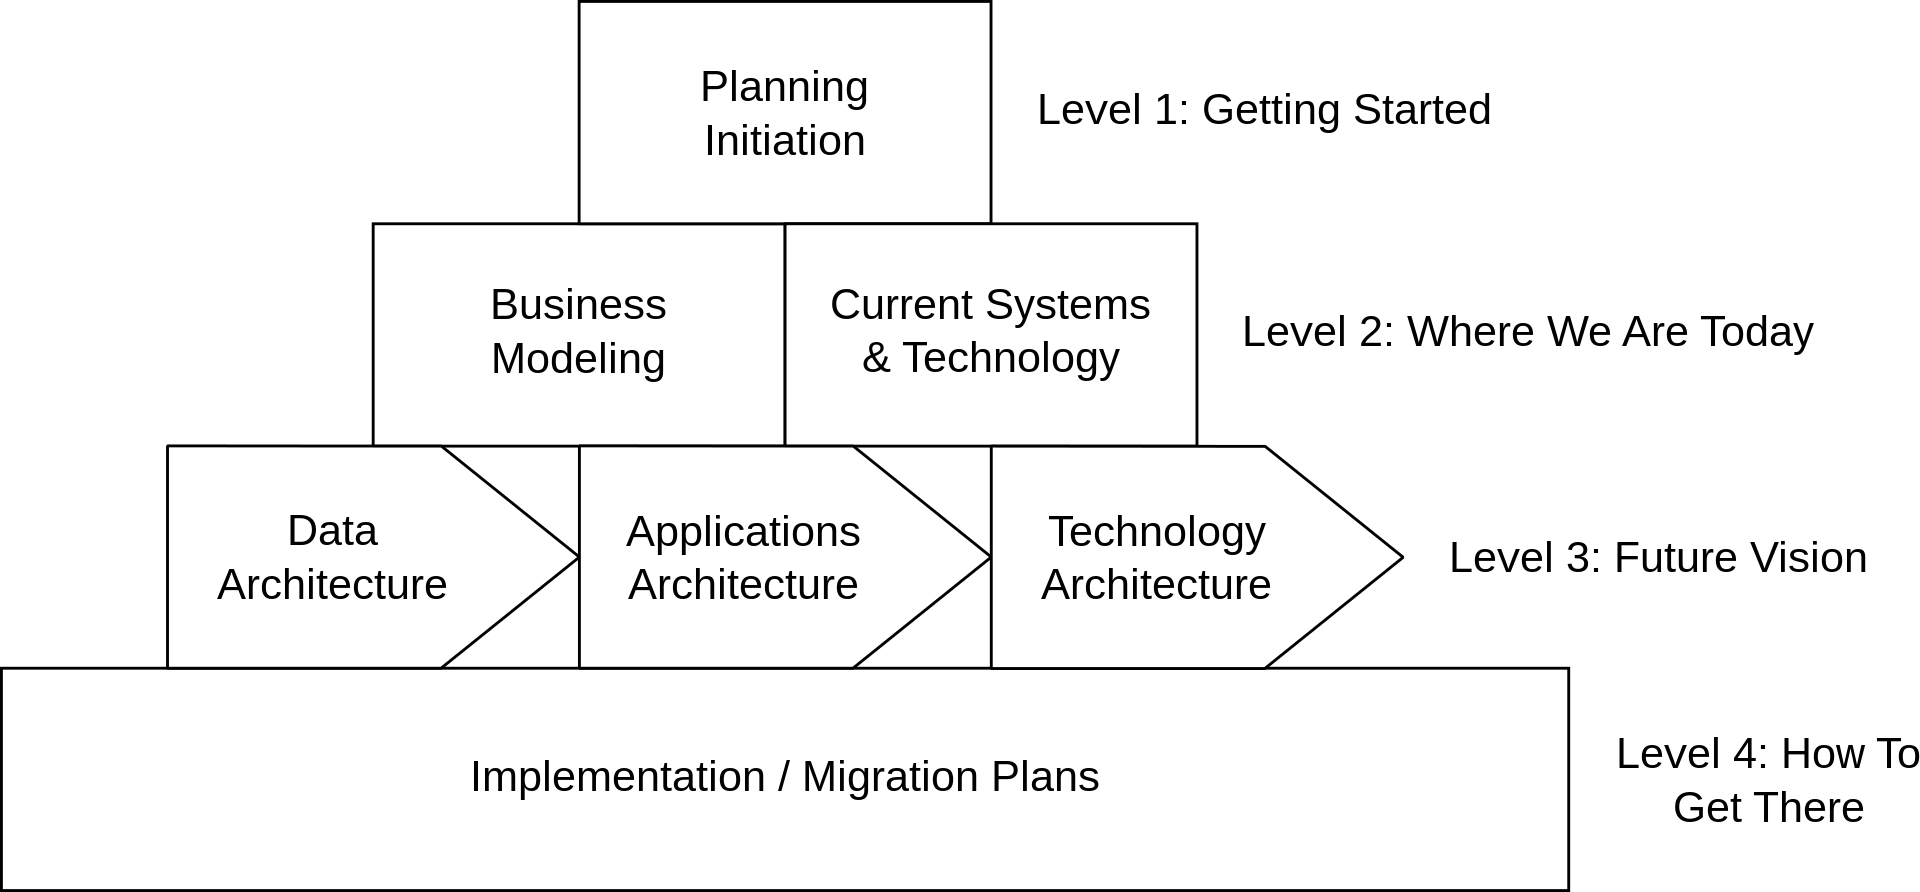
\includegraphics[width=1\textwidth]{../figures/eap}
\end{center}

\section{Sherwood Applied Business Security Architecture (SABSA)}
Sherwood Applied Business Security Architecture (SABSA) menyediakan model dan metodologi untuk mengembangkan kerangka kerja keamanan informasi dan manajemen risiko. SABSA dirancang dengan pendekatan "start-to-finish" dan "top-down" dan dapat disesuaikan dengan kebutuhan spesifik organisasi.

\begin{center}
	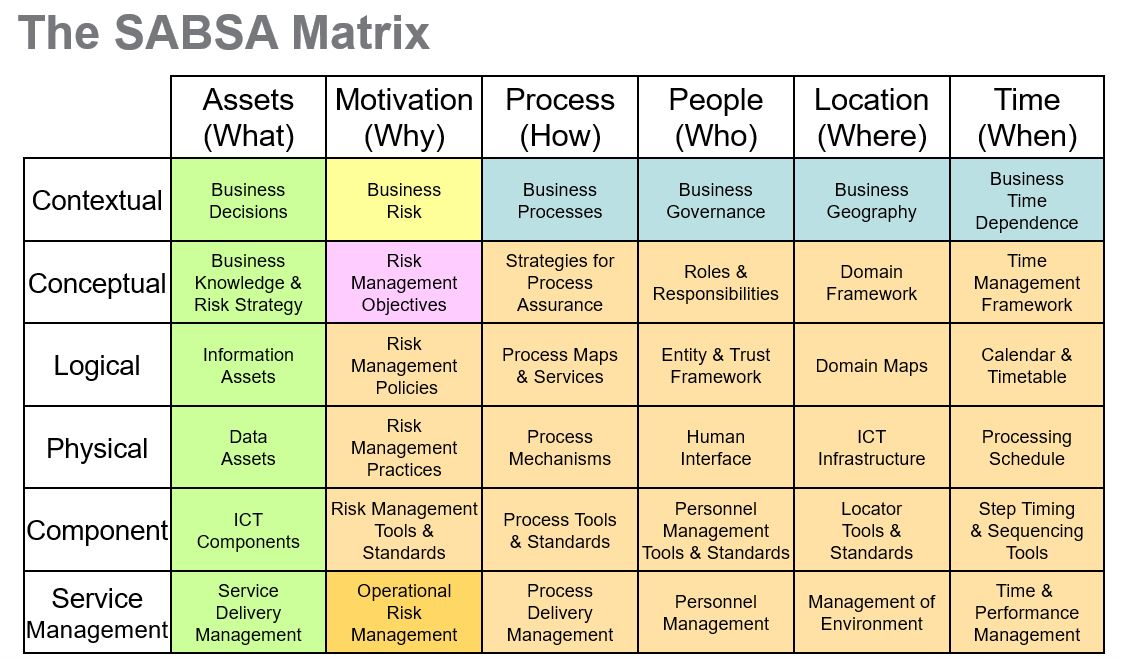
\includegraphics[width=0.8\textwidth]{../figures/sabsa}
\end{center}

\section{Federal Enterprise Architecture Framework (FEAF)}
Federal Enterprise Architecture Framework (FEAF) adalah kerangka kerja yang digunakan oleh pemerintah federal AS. FEAF membantu dalam meningkatkan efisiensi dan efektivitas layanan pemerintah, memfasilitasi kolaborasi antara agen dan departemen pemerintah, dan merupakan bagian dari strategi modernisasi TI pemerintah AS.

\begin{center}
	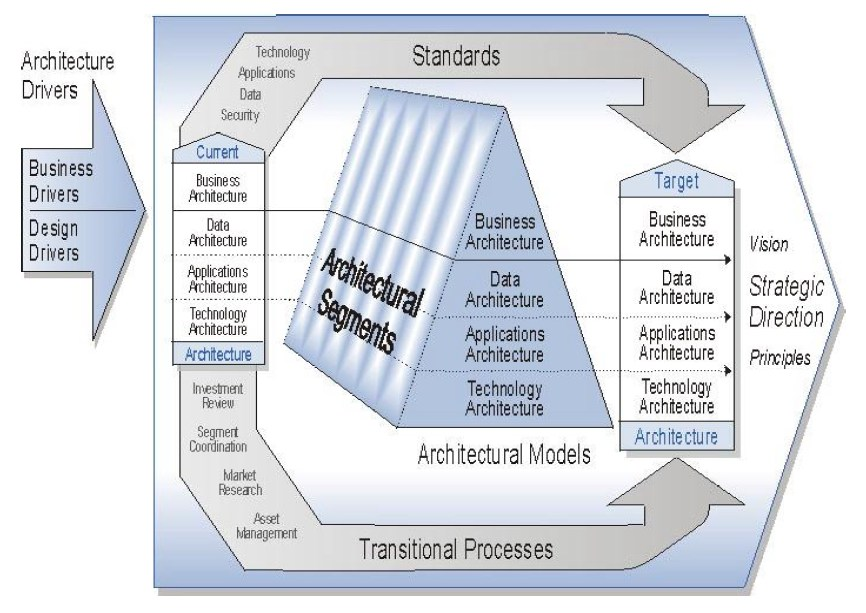
\includegraphics[width=.75\textwidth]{../figures/feaf}
\end{center}

\section{Gartner Enterprise Architecture Method}
Gartner Enterprise Architecture Method dikembangkan oleh perusahaan riset dan konsultasi Gartner. Metode ini membimbing organisasi dalam merancang, mengembangkan, dan menerapkan arsitektur enterprise, menghubungkan strategi bisnis dan TI, serta membantu organisasi mencapai tujuan transformasi digital mereka.

\begin{center}
	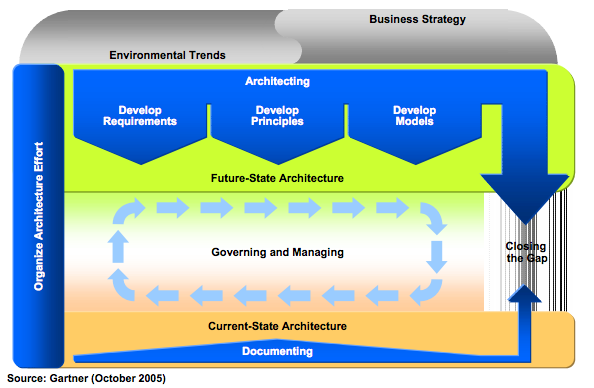
\includegraphics[width=.70\textwidth]{../figures/gartner}
\end{center}

\section{Department of Defense Architecture Framework (DoDAF)}
Department of Defense Architecture Framework (DoDAF) adalah kerangka kerja yang digunakan oleh Departemen Pertahanan AS. Kerangka ini membantu dalam mengorganisir dan memvisualisasikan informasi yang penting untuk proses pengambilan keputusan, menggunakan berbagai model dan panduan untuk mengembangkan arsitektur, dan cocok untuk organisasi dengan kompleksitas dan skala besar.

\begin{center}
	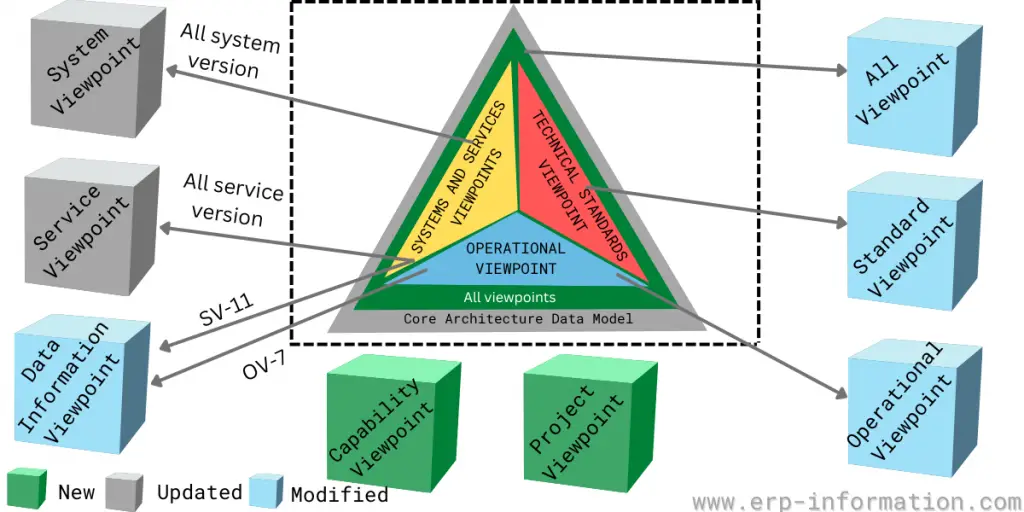
\includegraphics[width=0.68\textwidth]{../figures/dodaf}
\end{center}

\section{Australian Government AGA}
Australian Government AGA adalah kerangka kerja yang digunakan oleh Pemerintah Australia. Kerangka ini membantu dalam perencanaan dan implementasi teknologi informasi di tingkat pemerintah, mendorong kolaborasi antara departemen dan agen pemerintah, serta meningkatkan efisiensi dan transparansi layanan pemerintah.

\begin{center}
	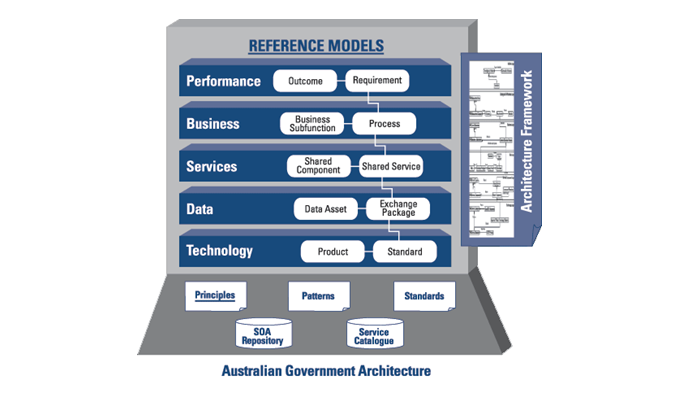
\includegraphics[width=0.9\textwidth]{../figures/aga}
\end{center}

\section{Business Architecture Body of Knowledge (BizBoK)}
Business Architecture Body of Knowledge (BizBoK) adalah panduan yang dikembangkan oleh Business Architecture Guild. Panduan ini menyediakan praktik terbaik dan standar dalam arsitektur bisnis, dapat digunakan oleh arsitek bisnis dan profesional terkait lainnya, serta membantu organisasi dalam merancang dan menerapkan arsitektur bisnis.

\begin{center}
	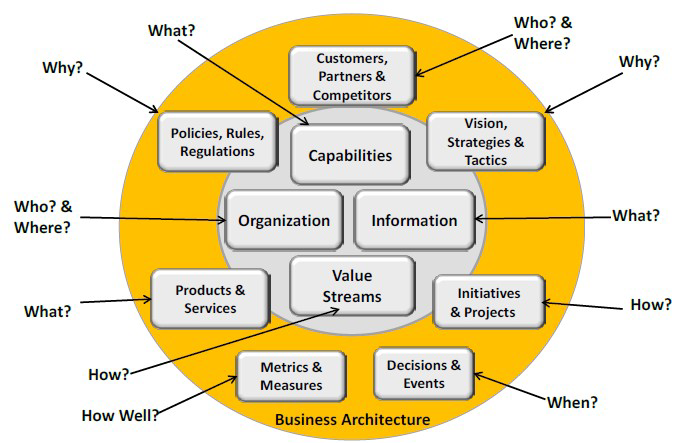
\includegraphics[width=0.7\textwidth]{../figures/bizbok}
\end{center}

\section{ISO Standard for Enterprise Modeling (ISO19439)}
ISO Standard for Enterprise Modeling (ISO19439) adalah standar internasional untuk pemodelan proses bisnis dan organisasi. Standar ini membantu dalam perencanaan, desain, dan perbaikan proses bisnis, dapat digunakan oleh berbagai jenis organisasi, dari bisnis hingga pemerintah, dan dikembangkan oleh Organisasi Internasional untuk Standardisasi (ISO).

\begin{center}
	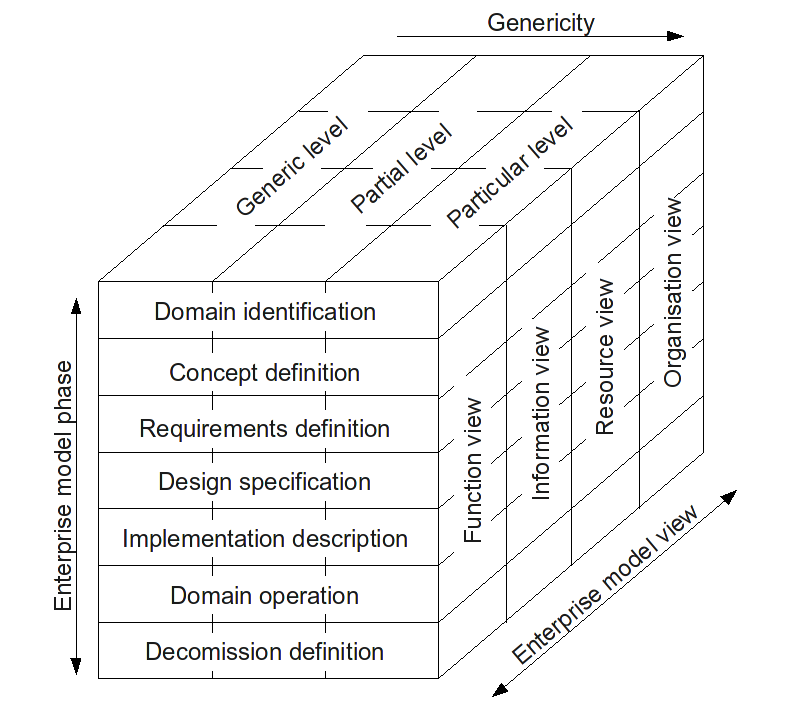
\includegraphics[width=.45\textwidth]{../figures/iso19439}
\end{center}

Terdapat berbagai kerangka dan metodologi arsitektur enterprise yang dapat dipilih sesuai dengan kebutuhan dan konteks spesifik organisasi. Arsitektur enterprise merupakan alat penting untuk perencanaan dan pengelolaan teknologi informasi dalam organisasi.

\section{Kesamaan Antar Kerangka Arsitektur Enterprise}
Meskipun terdapat berbagai kerangka arsitektur enterprise dengan pendekatan dan fokus yang berbeda, beberapa kesamaan mendasar dapat ditemukan di antara mereka:

\begin{itemize}
	\item \textbf{Pendekatan Terstruktur:} Semua kerangka arsitektur enterprise menerapkan pendekatan terstruktur untuk merancang dan mengelola sistem informasi dan TI. Mereka membagi arsitektur menjadi berbagai komponen atau lapisan untuk membantu dalam perencanaan dan implementasi yang lebih baik.
	
	\item \textbf{Fokus pada Keselarasan Strategis:} Kerangka-kerangka ini menekankan pentingnya menyelaraskan teknologi informasi dengan tujuan bisnis organisasi. Mereka berusaha memastikan bahwa keputusan TI mendukung dan memperkuat strategi bisnis keseluruhan.
	
	\item \textbf{Peningkatan Efisiensi dan Efektivitas:} Salah satu tujuan utama dari semua kerangka ini adalah meningkatkan efisiensi dan efektivitas operasional organisasi. Mereka berusaha mengoptimalkan penggunaan sumber daya dan mengurangi kompleksitas dengan memberikan panduan yang jelas dan metodologi yang teruji.
	
	\item \textbf{Manajemen Kompleksitas:} Kerangka-kerangka ini dirancang untuk membantu organisasi dalam mengelola kompleksitas sistem TI dan proses bisnis. Mereka memberikan struktur dan alat untuk memetakan, menganalisis, dan mengelola berbagai aspek arsitektur enterprise.
	
	\item \textbf{Pendekatan Berbasis Model:} Sebagian besar kerangka arsitektur menggunakan model atau representasi visual untuk menggambarkan arsitektur enterprise. Ini membantu dalam memahami hubungan antara berbagai komponen dan bagaimana mereka berinteraksi satu sama lain.
	
	\item \textbf{Fleksibilitas dan Penyesuaian:} Banyak kerangka arsitektur memungkinkan penyesuaian untuk memenuhi kebutuhan spesifik organisasi. Mereka dirancang agar fleksibel dan dapat diterapkan di berbagai konteks dan industri, dari bisnis hingga pemerintahan.
	
	\item \textbf{Penggunaan dalam Perencanaan Strategis:} Kerangka-kerangka ini sering digunakan dalam perencanaan strategis untuk membantu organisasi merumuskan dan mengimplementasikan rencana TI yang selaras dengan tujuan jangka panjang mereka.
\end{itemize}

Dengan kesamaan-kesamaan ini, kerangka arsitektur enterprise memberikan panduan yang kuat untuk organisasi dalam mengelola dan merancang sistem informasi yang efektif dan efisien, meskipun dengan pendekatan dan metode yang berbeda.

\section{Perbedaan Antar Kerangka Arsitektur Enterprise}
Meskipun ada kesamaan di antara berbagai kerangka arsitektur enterprise, perbedaan penting juga ada di antara mereka, yang mencerminkan fokus, metodologi, dan tujuan yang berbeda. Berikut adalah beberapa perbedaan utama:

\begin{itemize}
	\item \textbf{Pendekatan dan Fokus:} Setiap kerangka arsitektur memiliki pendekatan dan fokus yang unik. Misalnya, Framework Zachman menawarkan kerangka kerja berbasis model yang sangat terstruktur untuk manajemen kompleksitas arsitektur, sementara SABSA berfokus pada keamanan dan manajemen risiko dalam konteks arsitektur enterprise.
	
	\item \textbf{Lapisan dan Komponen:} Kerangka arsitektur enterprise dapat memiliki lapisan dan komponen yang berbeda. Sebagai contoh, NIST Enterprise Architecture Model membagi arsitektur TI menjadi lima lapisan yang berbeda, sedangkan Zachman Framework menggunakan enam level berbeda untuk memahami arsitektur dari sudut pandang yang lebih luas.
	
	\item \textbf{Metodologi Pengembangan:} Beberapa kerangka mengikuti metodologi pengembangan tertentu. Misalnya, EAP (Enterprise Architecture Planning) lebih fokus pada perencanaan dan implementasi teknologi baru berdasarkan kebutuhan bisnis, sedangkan Gartner's Enterprise Architecture Method memberikan panduan untuk desain dan implementasi yang berhubungan erat dengan strategi bisnis.
	
	\item \textbf{Penggunaan Model dan Visualisasi:} Setiap kerangka memiliki cara berbeda dalam menggunakan model dan visualisasi. PRISM Architecture Framework, misalnya, menggunakan matriks dan hubungan untuk menggambarkan arsitektur, sementara DoDAF (Department of Defense Architecture Framework) menggunakan berbagai model untuk mendukung proses pengambilan keputusan yang kompleks.
	
	\item \textbf{Aplikasi Sektor dan Konteks:} Beberapa kerangka lebih ditujukan untuk konteks atau sektor tertentu. FEAF (Federal Enterprise Architecture Framework) dirancang khusus untuk pemerintah federal AS, sedangkan Australian Government AGA adalah kerangka kerja yang dirancang untuk meningkatkan efisiensi dan transparansi di tingkat pemerintahan Australia.
	
	\item \textbf{Fleksibilitas dan Penyesuaian:} Derajat fleksibilitas dan penyesuaian juga bervariasi. Beberapa kerangka, seperti Zachman Framework, memiliki struktur yang sangat kaku, terperinci, dan befokus pada artefak, sementara yang lain, seperti SABSA, lebih mudah disesuaikan dengan kebutuhan spesifik keamanan organisasi untuk keperluan bisnis (\textit{business-centric security architectures} dan \textit{risk management frameworks}).
	
	\item \textbf{Standar Internasional:} Kerangka seperti ISO19439 memiliki standar internasional yang mendefinisikan model dan metode untuk perencanaan dan desain proses bisnis, yang mungkin berbeda dengan pendekatan spesifik yang diadopsi oleh kerangka lain.
\end{itemize}

Perbedaan-perbedaan ini mencerminkan variasi dalam kebutuhan organisasi dan konteks di mana kerangka arsitektur diterapkan. Memahami perbedaan ini membantu organisasi memilih kerangka yang paling sesuai dengan tujuan dan tantangan mereka.

\section{Deskripsi Tugas Mata Kuliah Enterprise Architecture}
Untuk membantu kelulusan, mahasiswa diharapkan dapat menghasilkan makalah ilmiah di akhir perkuliahan 1 semester. Model yang dipakailah adalah model flipped classroom di mana mahasiswa akan aktif berpartisipasi dalam perkuliahan. Misalnya, dengan mempresentasikan kemajuan tugas untuk berdiskusi dan mendapatkan umpan balik dari peserta kelas lainnya.

\begin{enumerate}
	\item \textbf{Sesi-01: Introduction to Enterprise Architecture} \\
	\textbf{Tugas}: Identifikasi satu masalah atau peluang di tempat kerja Anda. Anda bisa menggunakan alat-alat analisis seperti SWOT (Strength, Weakness, Opportunity, Threat), Porter's Five Forces, PESTLE (Political, Economic, Social, Technological, Legal, Environmental) ,dsb. Temukan teknologi/inovasi yang dapat meningkatkan kualitas tempat kerja Anda. Identifikasi visi dan misi organisasi tempat Anda bekerja. Wawancarai anggota dewan (\textit{board}), manajer, rekan kerja, atau pihak lain di organisasi tersebut.  Diskusikan ide-ide Anda dengan mereka dan catat umpan balik mereka. Mereka mungkin memberikan ide alternatif atau tambahan. Berdasarkan temuan-temuan ada pada tugas pertemuan sebelumnya, tetapkan \textbf{kemampuan} apa yang perlu ditambahkan ke perusahaan Anda bekerja untuk meningkatkan kualitas bisnisnya. Jadikan itu sebagai studi kasus Anda dan kembangkan arsitektur perusahaan selama semester ini. Ceritakan temuan Anda dalam template makalah.
	
	
	\item \textbf{Sesi-02: Studi Kasus - Remote Working (atau Masalah Lainnya)} \\
	\textbf{Tugas}: 1.) Baca literatur yang membahas TOGAF. 2.) Berdasarkan temuan-temuan ada pada tugas pertemuan sebelumnya, tetapkan \textbf{kemampuan} apa yang perlu ditambahkan ke perusahaan Anda bekerja untuk meningkatkan kualitas bisnisnya. Selanjutlnya, temukan setidaknya 30 sumber pustaka, termasuk makalah akademik, laporan, white papers, dll.
	
	
	\item \textbf{Sesi-03: TOGAF} \\
	\textbf{Tugas}: Lakukan studi literatur terkait visi Anda. Baca setidaknya 30 sumber, termasuk makalah akademik, laporan, white papers, dll., yang sudah Anda kumpulkan sebelumnya.
	
	\item \textbf{Sesi-04: Preliminary Phase} \\
	\textbf{Tugas}: Definisikan visi, yang sering dibagi menjadi tujuan atau sasaran, berdasarkan informasi yang dikumpulkan dalam fase Preliminary. Deskripsikan keadaan saat ini (As-Is) dan keadaan target (To-Be) untuk memperjelas visi tersebut.
	
	\item \textbf{Sesi-05: Phase A - Architecture Vision} \\
	\textbf{Tugas}: Buat model alur kerja/proses bisnis \textbf{As-Is} yang terpengaruh oleh visi. Juga, buat model alur kerja/proses bisnis \textbf{To-Be} yang diperlukan untuk mewujudkan visi tersebut. Identifikasi kesenjangan dan tindakan yang perlu diambil.
	
	\item \textbf{Sesi-06: Phase B - Business Architecture} \\
	\textbf{Tugas}: Buat model data dan dokumen \textbf{As-Is} yang terpengaruh oleh visi dan proses bisnis/workflows As-Is. Selain itu, buat model data dan dokumen \textbf{To-Be} yang diperlukan untuk mewujudkan visi tersebut dan proses bisnis/workflows To-Be. Identifikasi kesenjangan dan tindakan yang diperlukan.
	
	\item \textbf{Sesi-07: Phase C - Data Architecture} \\
	\textbf{Tugas}: Buat model aplikasi \textbf{As-Is} yang terpengaruh oleh visi, proses bisnis/workflows As-Is, dan model data dan dokumen As-Is. Juga, buat model aplikasi \textbf{To-Be} yang diperlukan untuk mewujudkan visi, termasuk proses bisnis/workflows To-Be dan model data dan dokumen To-Be. Identifikasi kesenjangan dan tindakan yang diperlukan.
	
	\item \textbf{Sesi-08: Phase C - Application Architecture} \\
	\textbf{Tugas}: Buat model infrastruktur/teknologi \textbf{As-Is} yang terpengaruh oleh visi, proses bisnis/workflows As-Is, model data dan dokumen As-Is, dan model aplikasi As-Is. Juga, buat model infrastruktur/teknologi \textbf{To-Be} yang diperlukan untuk mewujudkan visi, termasuk proses bisnis/workflows To-Be, model data dan dokumen To-Be, dan model aplikasi To-Be. Identifikasi kesenjangan dan tindakan yang diperlukan.
	
	\item \textbf{Sesi-09: Phase D - Technology Architecture} \\
	\textbf{Tugas}: Kelompokkan tindakan dari sesi sebelumnya ke dalam paket kerja dan estimasikan biaya (termasuk jadwal, tenaga kerja, dan sumber daya lainnya) untuk pelaksanaannya. Identifikasi peluang untuk mengoptimalkan pelaksanaan (misalnya, urutan paket kerja, penggabungan tindakan untuk mengurangi biaya).
	
	\item \textbf{Sesi-10: Phase E - Opportunities and Solutions} \\
	\textbf{Tugas}: Tuliskan semua pekerjaan Anda dan hasilkan makalah akademik (Shinta 2).
	
	\item \textbf{Sesi-11: Phase F - Migration Planning} \\
	\textbf{Tugas}: Tuliskan semua pekerjaan Anda dan hasilkan makalah akademik (Shinta 2).
	
	\item \textbf{Sesi-12: Phase G - Implementation Governance} \\
	\textbf{Tugas}: Tuliskan semua pekerjaan Anda dan hasilkan makalah akademik (Shinta 2).
	
	\item \textbf{Sesi-13: Phase H - Architecture Change Management} \\
	\textbf{Tugas}: Tuliskan semua pekerjaan Anda dan hasilkan makalah akademik (Shinta 2). \textbf{Ubah makalah Anda ke dalam bahasa Inggris.}
	
	\item \textbf{Sesi-14: Requirements Management}. Tidak ada tugas
\end{enumerate}


\section{Aktivitas Kelas dan Tugas}
Identifikasi satu masalah atau peluang di tempat kerja Anda. Anda bisa menggunakan alat-alat analisis seperti SWOT (Strength, Weakness, Opportunity, Threat), Porter's Five Forces, PESTLE (Political, Economic, Social, Technological, Legal, Environmental) ,dsb. Temukan teknologi/inovasi yang dapat meningkatkan kualitas tempat kerja Anda.

Identifikasi visi dan misi organisasi tempat Anda bekerja. Wawancarai anggota dewan (\textit{board}), manajer, rekan kerja, atau pihak lain di organisasi tersebut. Diskusikan ide-ide Anda dengan mereka dan catat umpan balik mereka. Mereka mungkin memberikan ide alternatif atau tambahan. Pilih salah satu sebagai studi kasus Anda dan kembangkan arsitektur perusahaan selama semester ini. Ceritakan temuan Anda dalam template makalah. Template makalah bisa didapatkan di: \url{https://journal.unnes.ac.id/nju/index.php/sji/about/editorialPolicies#focusAndScope}. Klik pada tautan \href{https://docs.google.com/document/d/13pIvz0OUnRtcnNZAcdfQGST5BSpx7LA3/edit}{\textsf{Template Article}}.
